 
\section{Experiments}

 
\subsection{Setup}

 
\paragraph{Explorers.}
We evaluate explorers from four families. Two \emph{baselines} bound the dynamic range: Oracle returns $R_{\text{core}}$ directly, and Random returns uniformly sampled regions. \emph{Sparse retrievers} are represented by BM25~\citep{robertson2009bm25} and TF--IDF~\citep{salton1988termweighting}. As a \emph{lightweight dense retriever} we use a RAG pipeline instantiated with Potion, a static word-embedding retriever distilled from a sentence transformer. Finally, the \emph{agentic explorers} cover five general-purpose coding agents (Claude Code~\citep{anthropic2025claudecode}, Codex, OpenHands~\citep{wang2024openhands}, Mini-SWE-Agent~\citep{yang2024sweagent}, AweAgent~\citep{chen2026beyondswecurrentcodeagent}) and four published academic localization agents (AutoCodeRover~\citep{zhang2024autocoderover}, LocAgent~\citep{chen2025locagent}, OrcaLoca~\citep{yu2025orcaloca}, CoSIL~\citep{jiang2025issuelocalizationllmdriveniterative}); Oracle in particular plays a central role in validating our ground-truth construction (\S\ref{sec:downstream}).


 
\paragraph{Metrics.} Following the analysis in \S\ref{sec:metrics}, we report a combination of strongly predictive metrics and standard baselines. The primary metrics are Precision, nDCG@500, HitFile, and Context Efficiency, selected for their high correlation with downstream behavior and low mutual redundancy. We additionally report Recall, F1, and hit/noise region rates as conventional references, even though several of these exhibit weaker predictive power individually. Full metric definitions are in \S\ref{sec:metrics}.

 
\paragraph{Choice of $K$.}
On our refined ground truth, the per-instance number of core regions averages roughly $4.7$ after the LLM-refinement step (\S\ref{sec:gt}). We therefore fix $K{=}5$ for every explorer in this paper: each explorer is asked to return its five most relevant regions, which keeps the comparison both fair across systems and aligned with the size of the supervision target.















\begin{table}[t]
  \centering
  % ---------- left: downstream resolve rate ----------
  \begin{minipage}[t]{0.46\linewidth}
    \vspace{0pt}
    \centering
    \captionof{table}{Downstream resolve rate under the restricted-context
    validation environment (GPT-5.4 with Mini-SWE-Agent, $K{=}5$).}
    \label{tab:downstream}
    \vspace{1mm}
    \footnotesize
\renewcommand{\arraystretch}{1.15}
\begin{tabular}{@{} l c @{}}
  \toprule
  Explorer & Resolve Rate (\%) \\
  \midrule
  Oracle             & 59.7 \\
  Random             &  4.7 \\
  \midrule
  TF-IDF             & 26.0 \\
  RAG                & 23.3 \\
  BM25               & 12.7 \\
  \midrule
  CoSIL              & 59.3 \\
  Mini-SWE-Agent     & 50.0 \\
  Openhands          & 47.7 \\
  OrcaLoca           & 45.3 \\
  AutoCodeRover      & 44.7 \\
  LocAgent           & 44.7 \\
  AweAgent           & 41.3 \\
  \midrule
  Codex              & 50.3 \\
  Claude Code        & 48.0 \\
  \bottomrule
\end{tabular}

  \end{minipage}\hfill
  % ---------- right: metric correlation ----------
  \begin{minipage}[t]{0.51\linewidth}
    \vspace{0pt}
    \centering
    \captionof{table}{Explorer-level correlation between each upstream
    exploration metric and downstream resolve rate, computed across all
    explorers in our pool. $\downarrow$ marks lower-is-better.}
    \label{tab:correlation}
    \vspace{1mm}
    \footnotesize
\renewcommand{\arraystretch}{1.12}
\setlength{\tabcolsep}{6pt}
\begin{tabular}{@{} l cc @{}}
  \toprule
  Metric & Pearson $r$ & Spearman $\rho$ \\
  \midrule
  CtxEff                 & $+0.950$ & $+0.739$ \\
  FUH                    & $+0.928$ & $+0.675$ \\
  Rec@100                & $+0.926$ & $+0.845$ \\
  HitFile                & $+0.925$ & $+0.695$ \\
  nDCG@500               & $+0.921$ & $+0.460$ \\
  nDCG@300               & $+0.920$ & $+0.458$ \\
  nDCG@100               & $+0.917$ & $+0.480$ \\
  HitReg                 & $+0.901$ & $+0.695$ \\
  Prec                   & $+0.890$ & $+0.671$ \\
  NoiseReg $\downarrow$  & $-0.812$ & $-0.562$ \\
  NoiseFile $\downarrow$ & $-0.808$ & $-0.590$ \\
  Rec@300                & $+0.769$ & $+0.796$ \\
  Rec@500                & $+0.710$ & $+0.796$ \\
  F1                     & $+0.673$ & $+0.810$ \\
  Rec$_\ell$             & $+0.617$ & $+0.796$ \\
  \bottomrule
\end{tabular}

  \end{minipage}
  \vspace{-2mm}
\end{table}





%
\begin{table*}[t]
  \centering
  \caption{Exploration quality at $K{=}5$ across different LLMs powering the same \textbf{Mini-SWE-Agent} scaffold. \textbf{Bold} marks the best result per column; \underline{underline} marks the second best.}
  \label{tab:llm-comparison}
  \vspace{1mm}
  \scriptsize
  \renewcommand{\arraystretch}{1.15}
  \begin{tabular*}{\textwidth}{@{\extracolsep{\fill}} l cccc c ccc cc @{}}
    \toprule
    & \multicolumn{5}{c}{\textit{Coverage \& Accuracy}} & \multicolumn{3}{c}{\textit{Ranking}} & \multicolumn{2}{c}{\textit{Efficiency \& Noise}} \\
    \cmidrule(lr){2-6} \cmidrule(lr){7-9} \cmidrule(lr){10-11}
    Model
      & HitReg & Prec & Rec$_\ell$ & F1 & HitFile
      & nDCG@500 & Rec@500 & FUH
      & CtxEff & NoiseReg$\downarrow$ \\
    \midrule
    GPT-5.4
      & \underline{0.516} & \textbf{0.542} & \underline{0.154} & \underline{0.194} & \textbf{0.655}
      & \underline{0.905} & \underline{0.154} & \underline{0.927}
      & \textbf{0.771} & \textbf{0.258} \\
    GPT-5.4-mini
      & \textbf{0.531} & 0.509 & \textbf{0.185} & \textbf{0.215} & \underline{0.649}
      & \textbf{0.924} & \textbf{0.183} & \textbf{0.956}
      & \underline{0.754} & \underline{0.265} \\
    Kimi-K2.6
      & 0.413 & 0.475 & 0.117 & 0.149 & 0.509
      & 0.739 & 0.115 & 0.759
      & 0.676 & 0.316 \\
    Sonnet-4.5
      & 0.428 & \underline{0.519} & {0.118} & 0.154 & 0.535
      & 0.779 & 0.116 & 0.802
      & 0.715 & 0.279 \\
    GLM-4.7
      & 0.289 & 0.414 & 0.122 & 0.148 & 0.343 & 0.557 & 0.105 & 0.572 & 0.536 & 0.465 \\
    Gemini-3-Pro
      & 0.268 & 0.420 & 0.052 & 0.079 & 0.369 & 0.605 & 0.052 & 0.620 & 0.540 & 0.467 \\
    \bottomrule
  \end{tabular*}
  \vspace{-4mm}
\end{table*}




 
\subsection{Downstream validation.}
\label{sec:downstream}
 


Before using upstream exploration metrics as the main evaluation target, we ask whether they track downstream repair behavior. On a shared $n{=}150$ subset of SWE-Explore Bench, each explorer provides its $K{=}5$ ranked regions; the resulting context is then given to a fixed Mini-SWE-Agent patcher backed by GPT-5.4 and Gemini-3-Pro, and we average the SWE-bench harness resolve rate over the two patchers. Table~\ref{tab:correlation} reports the explorer-level Pearson and Spearman correlations between each upstream metric and this downstream resolve rate.
 
\paragraph{Stable signals.}
The strongest metrics are not purely file-level or purely recall-based. Context Efficiency has the highest Pearson correlation ($r{=}0.950$), suggesting that useful context must be both relevant and compact. Rec@100 is the strongest rank-correlated signal ($\rho{=}0.845$), indicating that early coverage under a tight line budget is especially predictive of repair. HitFile, HitRegion, and FUH remain strong Pearson signals: they capture whether the explorer reaches the right file, overlaps the right evidence, and surfaces useful evidence early. Precision is also predictive, but it is most informative when interpreted together with coverage-oriented metrics.

 
\paragraph{Useful but incomplete signals.}
Rank-aware metrics such as nDCG@500 have very high Pearson correlation but weaker Spearman correlation, indicating that they separate broad quality tiers well but are less stable for ordering nearby explorers. Recall-style metrics show a budget effect: Rec@100 is strong in both views, while broader recall metrics and F1 are more rank-sensitive than scale-sensitive, reflecting their tendency to reward broad reading even when the selected context is not compact. Noise rates have the expected negative correlation, but serve better as diagnostics than as standalone success measures. Together, these results justify reporting a mixed metric set rather than a single score. In Table~\ref{tab:main-results} and Table~\ref{tab:llm-comparison}, we therefore emphasize HitRegion, HitFile, Precision, nDCG@500, FUH, and Context Efficiency, while retaining Recall, F1, Recall@500, and noise-region rate as complementary diagnostics.














\begin{table*}[t]
  \centering
  \caption{Exploration quality at $K{=}5$. \textbf{Bold} marks the best non-oracle result per column; \underline{underline} marks the second best. HitReg / HitFile are region-/file-level hit rates; Rec$_\ell$ is line-level recall. $\downarrow$ indicates lower is better; all others are higher-is-better. All agentic explorers are driven by GPT-5.4 as the underlying model.}
  
  \label{tab:main-results}
  \vspace{1mm}
  \scriptsize
  \renewcommand{\arraystretch}{1.10}
  \setlength{\tabcolsep}{4pt}
  \begin{tabular*}{\textwidth}{@{\extracolsep{\fill}} l ccccc ccc cc @{}}
    \toprule
    & \multicolumn{5}{c}{\textit{Coverage \& Accuracy}} & \multicolumn{3}{c}{\textit{Ranking}} & \multicolumn{2}{c}{\textit{Efficiency \& Noise}} \\
    \cmidrule(lr){2-6} \cmidrule(lr){7-9} \cmidrule(lr){10-11}
    Explorer
      & HitReg & Prec & Rec$_\ell$ & F1 & HitFile
      & nDCG@500 & Rec@500 & FUH
      & CtxEff & NoiseReg$\downarrow$ \\
    \midrule
    Oracle  & 0.915 & 1.000 & 0.953 & 0.964 & 0.923 & 0.858 & 0.576 & 1.000 & 1.000 & 0.000 \\
    Random  & 0.003 & 0.002 & 0.004 & 0.002 & 0.004 & 0.004 & 0.001 & 0.006 & 0.002 & 0.997 \\
    \midrule
    BM25    & 0.065 & 0.055 & 0.021 & 0.024 & 0.079 & 0.132 & 0.021 & 0.141 & 0.087 & 0.910 \\
    TF-IDF  & 0.121 & 0.117 & 0.049 & 0.054 & 0.140 & 0.223 & 0.049 & 0.240 & 0.190 & 0.821 \\
    Potion  & 0.069 & 0.055 & 0.025 & 0.026 & 0.088 & 0.136 & 0.025 & 0.146 & 0.100 & 0.897 \\
    \midrule
    OpenHands      & 0.514 & 0.489 & 0.179 & 0.209 & 0.645 & 0.867 & 0.177 & 0.895 & 0.737 & 0.245 \\
    Mini-SWE-Agent & 0.505 & 0.530 & 0.151 & 0.190 & 0.640 & 0.885 & 0.151 & 0.907 & 0.754 & 0.253 \\
    AweAgent       & \underline{0.534} & 0.577 & 0.140 & 0.182 & \textbf{0.682} & \textbf{0.954} & 0.140 & \underline{0.975} & \underline{0.829} & 0.191 \\
    AutoCodeRover  & 0.272 & \textbf{0.680} & \underline{0.233} & \underline{0.291} & 0.280 & 0.720 & 0.165 & 0.730 & 0.738 & \underline{0.034} \\
    LocAgent       & 0.472 & \underline{0.642} & 0.191 & 0.241 & 0.540 & \underline{0.950} & 0.173 & \textbf{0.977} & 0.799 & 0.195 \\
    OrcaLoca       & 0.126 & 0.295 & 0.033 & 0.049 & 0.129 & 0.311 & 0.030 & 0.313 & 0.317 & \textbf{0.003} \\
    CoSIL          & \textbf{0.544} & 0.581 & \textbf{0.788} & \textbf{0.602} & 0.544 & 0.824 & \textbf{0.412} & 0.920 & \textbf{0.898} & 0.471 \\
    \midrule
    Claude Code    & 0.531 & 0.598 & 0.154 & 0.202 & \underline{0.667} & 0.938 & 0.154 & 0.963 & \underline{0.829} & 0.186 \\
    Codex          & 0.516 & 0.523 & 0.194 & 0.223 & 0.649 & 0.901 & \underline{0.190} & 0.936 & 0.762 & 0.249 \\
    \bottomrule
  \end{tabular*}
  \vspace{-4mm}
\end{table*}














% ────────────────────────────────────────────────────────────────────
% ────────────────────────────────────────────────────────────────────
 
\subsection{Exploration Quality}
\label{sec:main-results}
 
Table~\ref{tab:llm-comparison} and Table~\ref{tab:main-results} report upstream exploration quality for all explorers and models at $K{=}5$. We highlight the following observations.

 
\paragraph{Agentic exploration is a clear step above non-agentic retrieval.}
Sparse retrievers (BM25, TF--IDF) and the lightweight dense retriever remain close to Random on most metrics, while every agentic explorer is substantially higher than them. This confirms that repository exploration is not well captured by one-shot lexical or embedding retrieval alone: multi-step interaction with the repository is already necessary to reach the metric range occupied by modern coding agents.
 
\paragraph{Low F1 is mostly a recall problem.}
Despite strong file-level hit rates and ranking scores, most non-oracle explorers still have low F1, and the limiting term is usually line-level recall rather than precision. The general-purpose coding agents all reach high HitFile and nDCG@500, but their Rec$_\ell$ remains only around $0.14$--$0.19$; AutoCodeRover is highly precise, yet also recall-limited. This suggests that broad enough repository exploration remains a central bottleneck for current code-agent-style explorers: they often find plausible files early, but miss many of the specific spans needed to cover the full ground-truth context.

 
\paragraph{LLM choice shifts the operating point, but not the bottleneck.}
Table~\ref{tab:llm-comparison} controls the scaffold by running the same Mini-SWE-Agent explorer with different LLMs. The GPT-family models form the strongest tier, but with slightly different profiles: GPT-5.4 is cleaner and more compact, while GPT-5.4-mini surfaces more core regions and ranks useful evidence earlier. Kimi-K2.6 and Sonnet-4.5 form a middle tier, and GLM-4.7 and Gemini-3-Pro lag mainly in coverage and ranking. The larger pattern is more important than the exact ordering: across all LLMs, file-level hits remain much stronger than line-level recall, so replacing the base model alone does not remove the exploration bottleneck. High-recall region discovery still appears to require better exploration mechanisms, not just a stronger patching model.

 
\paragraph{General coding agents behave surprisingly similarly.}
Claude Code, Codex, OpenHands, Mini-SWE-Agent, and AweAgent have closely matched profiles across coverage, ranking, and efficiency metrics. This is notable because they differ in implementation and harness complexity, yet their exploration outputs occupy nearly the same operating point: high file hit, high early ranking, compact context, and low line recall. The similarity suggests that a complex repair harness is not necessarily required to study the exploration subproblem; a simpler explorer interface can expose much of the same behavior.

 
\paragraph{Specialized localizers only help when they broaden search.}
The academic agents do not uniformly dominate general coding agents. AutoCodeRover is precise but conservative, OrcaLoca has very low noise but misses many relevant regions, and LocAgent resembles the general-agent profile rather than changing the recall frontier. CoSIL is the main exception: it achieves by far the highest non-oracle Rec$_\ell$ and F1, suggesting that its iterative code-graph search is an important component for high-recall exploration. In contrast, explorers that rely more heavily on shell-style navigation or narrow search actions may reach the right files while still under-covering line-level evidence.

\paragraph{Line-level evaluation adds information beyond file hits.}
HitFile remains a strong and useful signal, as shown by the downstream correlations in \S\ref{sec:downstream}; however, it does not distinguish whether an explorer actually surfaces the relevant spans inside those files. The contrast between high HitFile and much lower Rec$_\ell$ across most agentic explorers supports SWE-Explore's line-level design: file-level localization captures reaching the right neighborhood, while line-level metrics measure whether the evidence needed by successful trajectories is actually exposed.






























% ────────────────────────────────────────────────────────────────────
\begin{figure}[t]
  \centering
  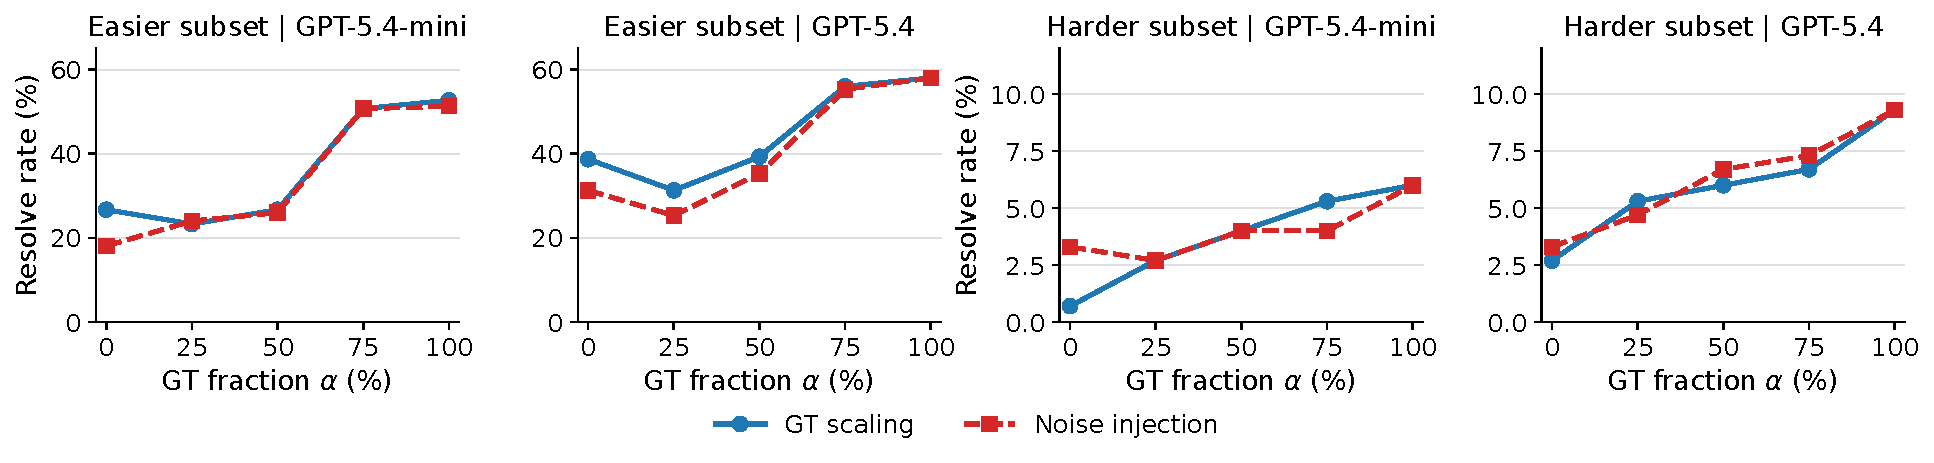
\includegraphics[width=0.95\linewidth]{paper/pictures/degradation_grid.pdf}
  \vspace{-2mm}
  \caption{Resolve rate as the visible context degrades from the Oracle's full core set $R_{\text{core}}$ to either $\alpha\%$ of $R_{\text{core}}$ alone (\emph{GT scaling}, solid) or $\alpha\%$ of $R_{\text{core}}$ padded back to full size with random non-core regions (\emph{noise injection}, dashed).}
  \label{fig:degradation}
\end{figure}
\vspace{-3mm}
\subsection{Controlled Context Degradation}
\label{sec:degradation}
\vspace{-1mm}
The previous sections show that explorer behavior differs along coverage, precision, ranking, and efficiency, and that these differences affect downstream repair. Here we ask a more controlled robustness question: is a patcher more sensitive to \emph{missing} relevant context or to \emph{redundant} irrelevant context? In the restricted-context validation environment (\S\ref{sec:bridge}), we synthetically perturb Oracle context by exposing only an $\alpha\in\{0,25,50,75,100\}$ fraction of core regions (missing-context condition), or by filling the removed budget with randomly sampled non-core regions (redundant-context condition). We sweep $\alpha$ on two stratified $n{=}150$ subsets of SWE-Explore under both a weak patcher GPT-5.4-mini and a strong patcher GPT-5.4; Figure~\ref{fig:degradation} reports all four panels.


\vspace{-3mm}
\paragraph{Missing context is the dominant failure mode.}
On the easier subset, downstream resolve rate changes sharply only after enough core evidence is present: performance stays low through partial context, then jumps between $\alpha{=}50$ and $\alpha{=}75$. This threshold-like pattern suggests that patchers are not simply accumulating value smoothly from every additional region; instead, several pieces of core evidence must be present together before a correct fix becomes likely. Redundant context is less damaging once this threshold is crossed: the redundant-context curve closely tracks the missing-context curve for $\alpha\geq75$, indicating that modern patchers can tolerate extra irrelevant code when the essential evidence is already visible. This agrees with the metric analysis above: in the high-coverage regime, missing core evidence matters more than moderate precision loss, so recall-oriented improvements are more valuable than small filtering gains. Redundancy hurts most when core evidence is scarce, especially at $\alpha{=}0$, where random non-core code lowers resolve rate by $7$--$9$\,pp. The harder subset shows a much narrower range, suggesting that when the issue itself exceeds the patcher's capability, improving context alone has limited effect.

\vspace{-3mm}
\paragraph{The easier-subset dip suggests caution with empty-context baselines.}
Both easier-subset curves dip from $\alpha{=}0$ to $\alpha{=}25$, especially under the stronger patcher. A plausible explanation is memorization: with no repository context, the model may rely on an issue-only prior, while a small incomplete slice of $R_{\text{core}}$ pushes it to reconcile partial evidence. Because the dip disappears on the harder subset, we treat it as a caveat rather than the main effect: empty-context baselines on canonical repositories may be inflated and should be interpreted carefully.


\section{Conclusion}

We presented \textbf{SWE-Explore}, a benchmark for evaluating repository exploration independently from patch generation through ranked, line-level context selection. Using trajectory-derived supervision, SWE-Explore compares retrievers, search agents, and long-context selectors by the evidence they surface rather than only by final repair outcomes. Our experiments show that exploration metrics track downstream repair, that current agents are strong at finding relevant files but remain recall-limited at the line level, and that missing core evidence hurts more than moderate redundant context. We hope SWE-Explore provides a focused target for building explorers that read repositories more broadly and expose the spans repair agents actually need.

